\subsubsection{UC19 - Configurazione alert}
\label{sssec:uc19}

\begin{figure}[h!]
  \begin{center}
    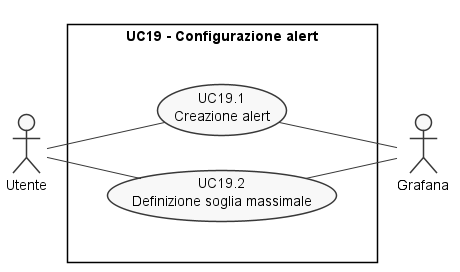
\includegraphics[width=10cm]{uc19.png}\\
    \caption{UC19 - Configurazione alert}%
    \label{fig:uc19}
  \end{center}
  \end{figure}

\begin{itemize}
  \item \textbf{Attore primario}: Utente;
  \item \textbf{Attore secondario}: Grafana;
  \item \textbf{Descrizione}: L'utente configura l'alert e imposta la soglia massimale;
  \item \textbf{Precondizione}:
  \begin{enumerate}
		\item L'utente ha configurato il plug-in correttamente(UC5);
		\item L'utente avvia il plug-in (UC14).
	\end {enumerate}
  \item \textbf{Scenario principale}:
  \begin{enumerate}
    \item L'utente definisce l'alert usando l'opzione "Crea alert"(UC19.1);
    \item L'utente definisce una soglia per l'alert appena creato, utilizzando i meccanismi offerti da Grafana(UC19.2).
  \end{enumerate}
  \item \textbf{Postcondizione}: L'utente ha impostato correttamente la soglia dell' alert.
\end{itemize}


\paragraph{UC19.1 - Creazione alert}
\label{para:uc19.1}
\begin{itemize}
  \item \textbf{Attore primario}: Utente;
  \item \textbf{Attore secondario}: Grafana;
  \item \textbf{Descrizione}: L'utente crea un alert usando l'opzione di creazione contenuta nel pannello di predizione;
  \item \textbf{Precondizione}: L'utente si trova sul pannello di predizione e il sistema permette di inserire un alert;
  \item \textbf{Scenario principale}: L'utente aggiunge un alert tramite l'opzione "Crea alert";
  \item \textbf{Postcondizione}: L'alert è stato creato.
\end{itemize}


\paragraph{UC19.2 - Definizione soglia massimale}
\label{para:uc19.2}
\begin{itemize}
  \item \textbf{Attore primario}: Utente;
  \item \textbf{Attore secondario}: Grafana;
  \item \textbf{Descrizione}: L'utente sceglie la soglia massimale per l'alert in creazione;
  \item \textbf{Precondizione}: L'utente ha a disposizione un alert(UC19.1);
  \item \textbf{Scenario principale}: L'utente tramite Grafana definisce la soglia per l'alert e invia la conferma della creazione del suddetto;
  \item \textbf{Postcondizione}: L'utente ha impostato la soglia in modo che parta l'alert tramite Grafana.
\end{itemize}
